\documentclass{article}

\usepackage{tikz}
\usetikzlibrary{math}

\begin{document}
    \begin{center}
        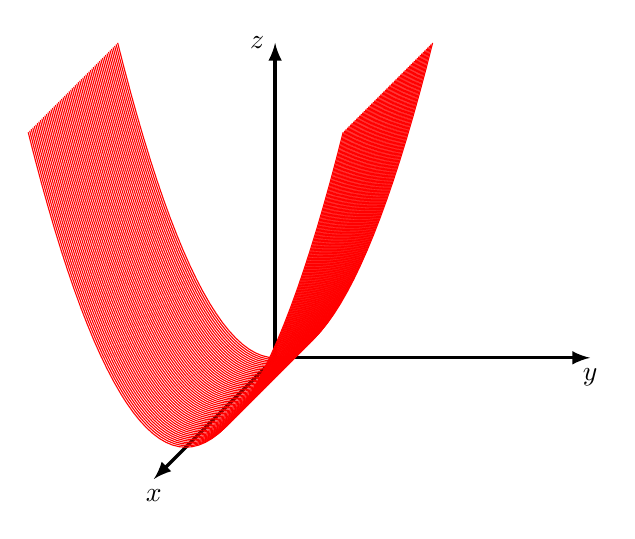
\begin{tikzpicture}
            \coordinate (O) at (0,0,0);
            \draw[very thick, ->, >=latex] (O) -- (4,0,0) node[below]{\(y\)};
            \draw[very thick, ->, >=latex] (O) -- (0,4,0) node[left]{\(z\)};
            \draw[very thick, ->, >=latex] (O) -- (0,0,4) node[below]{\(x\)};
            
            \foreach \z in {0,0.05, ..., 3}{
                \draw[red, domain=0:2] plot (\x,\x*\x,\z);
                \draw[red, domain=0:2] plot (-\x,\x*\x,\z);
            }
        \end{tikzpicture}

        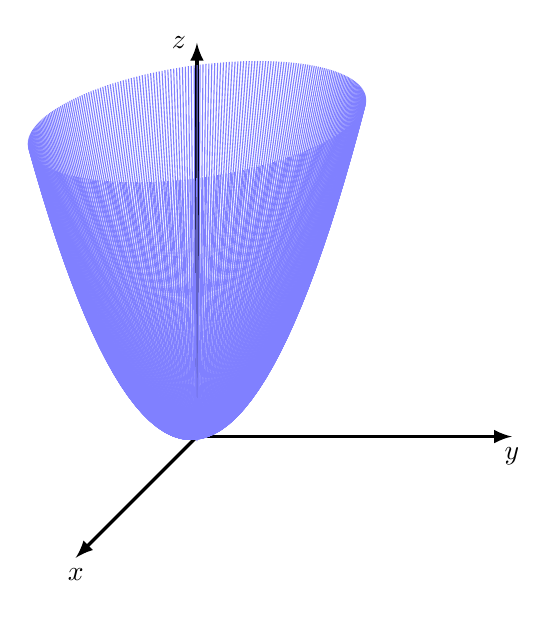
\begin{tikzpicture}
            \coordinate (O) at (0,0,0);
            \draw[very thick, ->, >=latex] (O) -- (4,0,0) node[below]{\(y\)};
            \draw[very thick, ->, >=latex] (O) -- (0,5,0) node[left]{\(z\)};
            \draw[very thick, ->, >=latex] (O) -- (0,0,4) node[below]{\(x\)};
            
            \foreach \angle in {0, ..., 360}{
                \draw[blue!50, rotate around y=\angle, domain=0:2] plot (\x,\x*\x, 0);
            }
        \end{tikzpicture}
    \end{center}
\end{document}